% !TeX encoding = UTF-8
% !TeX program = xelatex
% !TeX spellcheck = en_US

\documentclass[bachelor,arabic,pdf]{ustcthesis}
% doctor|master|bachelor [academic|professional] [chinese|english] [print|pdf]
% [super|numebers|authoryear]

\title{面向移动服务机器人的行人追踪跟随的研究与实现}
\author{韦清}
\major{计算机科学与技术}
\supervisor{陈小平\ 教授}
% \cosupervisor{钱学森\ 教授}
% \date{二〇一七年五月一日} % 注释掉则为今日
% \professionaltype{专业学位类型}
% \secretlevel{秘密}        % 绝密|机密|秘密,注释本行则不保密
% \secretyear{20}           % 保密年限

\entitle{Research and Implementation of People Tracking and Following with Mobile Service Robots}
\enauthor{Qing Wei}
\enmajor{Computer Science and Technology}
\ensupervisor{Prof. XIaoping Chen}
% \encosupervisor{Prof. Xuesen Qian}
% \endate{May 1, 2017}      % Today if commented
% \enprofessionaltype{Professional degree type}
% \ensecretlevel{Secret}    % Top secret|Highly secret|Secret


% 加载宏包和配置
\usepackage{graphicx}
\graphicspath{{figures/}}
\usepackage{booktabs}
\usepackage{longtable}
\usepackage[ruled,linesnumbered]{algorithm2e}
\usepackage{siunitx}
\usepackage{amsthm}
\usepackage{hyperref}

\DeclareRobustCommand\cs[1]{\texttt{\char`\\#1}}
\newcommand\pkg{\textsf}

\renewcommand\vec{\symbf}
\newcommand\mat{\symbf}
\newcommand\ts{\symbfsf}
\newcommand\real{\mathbf{R}}




\begin{document}

% 研究生论文:
%   封面,原创性声明和授权使用声明
%   frontmatter: 摘要,目录,[图、表清单],[符号说明]
%   mainmatter: 正文章节,参考文献
%   appendix: 附录
%   backmatter: 致谢,已发表论文列表
%
% 本科生论文:
%   封面
%   frontmatter: 致谢,目录,摘要
%   mainmatter: 正文章节,参考文献
%   appendix: 附录

\maketitle
\makestatement

\frontmatter
\tableofcontents
% !TeX root = ../main.tex

\begin{abstract}
  服务机器人是一种能完成有益于人类的服务工作的半自助或全自主型机器人,分为个人/家庭服务机器人和专业机器人。专业机器人一般在特定场景中使用,如商业服务、物流、医疗、救援等;而个人/家用服务机器人主要在日常生活场景中进行与人进行交互,提供家政服务、陪伴、娱乐、辅助学习等多种功能,包括家政机器人、娱乐休闲机器人、助老助残机器人等。其中,个人/家庭服务机器人为本文研究内容所适用的对象。

  随着人工智能与物联网技术迅速发展,个人家庭用机器人、公共服务机器人的应用场景、服务模式和市场也在不断拓展,成为了当下的一个研究热点。为了精准理解当前环境和有效执行指令,能够精确可靠地自动识别目标人物并对其进行追踪陪同,是这类移动服务机器人的人机交互中的一项重要且必要的功能。

  本文将针对室内移动机器人的行人跟随问题做如下三个方面的研究:

  (1)常用目标跟随算法的原理与实现:主要从行人检测和追踪两个角度进行调研论述。主要介绍了用于行人检测的几个常用特征,如颜色直方图、LBP、HOG、SIFT特征,基于机器学习的几种分类器,包括KNN、SVM、RandomForest、AdaBoost,以及几种常用的追踪算法,包括卡尔曼滤波、粒子滤波、均值漂移、相关滤波等。

  (2)ROS上的机器人导航技术;主要包括ROS提供的ROS导航包,以及中科大研发的可佳机器人的导航功能。

  (3)可佳机器人上行人跟随系统的实现;结合行人的HOG特征和HSV直方图特征,使用CSR-DCF算法进行行人追踪,并单独训练一个SVM分类器以防止追踪器发生误判/漏判,以及帮助追踪器从追踪失败中恢复。

  \keywords{计算机视觉;机器人;行人检测;目标追踪}
\end{abstract}

\begin{enabstract}
  A service robot is a robot which operates semi- or fully autonomously to perform services useful to the well-being of humans and equipment. They are capable of making decisions and acting autonomously in real and unpredictable environments to accomplish determined tasks.  There are two types of service robots, personal/domestic service robots and professional robots. Professional robots are typically used in specific occasions, including business, delivery, medical, rescue, etc. Personal/domestic service robots, which include cleaning robots, elder care and medical companions, entertainment and leisure robots, home education and training robots, are the specific application objects of the research in this paper.

  With the rapid development of artificial intelligence and IOT, the application scenarios, service patterns and market of service robots are also continuously expanding, thus making the service robots a focused area in Robotics research. In order to accurately understand the current environment and effectively execute the instructions, one of the important and necessary ability for a personal service robot, is to automatically recognize and track a person precisely and robustly.

  This paper is consist of three parts:

  (1) The theories and implementation of various existing object tracking algorithm;

  (2) Robot navigation on ROS;

  (3) The implementation of the people following system on kejia robot.

  \enkeywords{Computer Vision; Robotics; Pedestrian Detection; Object Tracking}
\end{enabstract}
% \listoffigures
% \listoftables
% !TeX root = ../main.tex

\begin{notation}

  \begin{notationlist}{2em}
    \item[$\displaystyle a$] The number of angels per unit area
    \item[$\displaystyle N$] The number of angels per needle point
    \item[$\displaystyle A$] The area of the needle point
    \item[$\displaystyle \sigma$] The total mass of angels per unit area
    \item[$\displaystyle m$] The mass of one angel
    \item[$\displaystyle \sum_{i=1}^n a_i$] The sum of $a_i$
  \end{notationlist}

\end{notation}



% 也可以使用 nomencl 宏包

% \printnomenclature

% \nomenclature{$\displaystyle a$}{The number of angels per unit are}
% \nomenclature{$\displaystyle N$}{The number of angels per needle point}
% \nomenclature{$\displaystyle A$}{The area of the needle point}
% \nomenclature{$\displaystyle \sigma$}{The total mass of angels per unit area}
% \nomenclature{$\displaystyle m$}{The mass of one angel}
% \nomenclature{$\displaystyle \sum_{i=1}^n a_i$}{The sum of $a_i$}


\mainmatter
% !TeX root = ../main.tex

\chapter{绪论}

\section{研究背景及意义}

  服务机器人是一种半自助或全自主工作的机器人。它能完成有益于人类健康的服务工作,但不包括从事生产的设备。它们可以在真实且不可预测的环境中自动进行决策和行动来完成确定的任务。服务机器人分为个人/家庭服务机器人和专业机器人。专业机器人一般在特定场景中使用,如商业服务、物流、医疗、救援等;而个人/家用服务机器人主要在日常生活场景中进行与人进行交互,提供家政服务、陪伴、娱乐、辅助学习等多种功能,包括家政机器人、娱乐休闲机器人、助老助残机器人等。其中,个人/家庭服务机器人为本文研究内容的应用对象。

  随着人工智能与物联网技术不断发展,服务机器人作为智能硬件之一,不断地丰富其自身功能及其实现更强大的性能,服务机器人市场也在迅速发展,家庭用机器人、智能公共服务机器人的应用场景和服务模式不断拓展。为了精准理解当前环境和有效执行指令,能够精确可靠地自动识别目标人物并对其进行追踪陪同,是这类移动服务机器人的人机交互中的一项重要且必要的功能。这项功能可以用于在博物馆或医院等场景中对用户进行指引,在家庭中陪伴用户、与用户进行交互,助老、助残等。

  移动机器人的核心技术包括导航定位、地图创建、路径规划、任务分配和目标跟踪等。在本文中,会主要介绍目标跟踪,尤其是其中的行人定位模块,通过对ROS导航的简要介绍涉及机器人导航定位、地图创建、路径规划的大致概念,并最终实现一个有简单导航模块和较为鲁棒的行人追踪模块的机器人系统。

\section{相关工作}

  自从有了服务机器人的概念以来,就有了很多对于机器人目标跟随技术的研究。移动机器人由于可携带多种传感器,由此衍生了各种使用了传感器的行人识别和追踪方法。如使用视觉图像、激光传感器、热成像传感器\cite{treptow2006real}、声音传感器\cite{zhou2008target}等,由于单一传感器信息较少,也出现了不少多传感器融合的行人定位方式\cite{susperregi2013rgb}。

  激光传感器由于还被广泛运用到机器人的定位、建图、导航中,是机器人最为重要的传感器,所以也最多地被运用到行人跟随的任务中。不过激光传感器由于成本限制,多使用2D激光检测同一水平面的物体,竖直空间上可以检测到的范围有限,所以激光行人追踪的方法最为经常使用的特征是行人的双腿\cite{arras2008efficient}。在激光图像中,人的双腿在有一种明显的模式,通过滤波器抽取人的腿部特征,进行聚类,便可得到一个人腿模式识别器,再结合粒子滤波或卡尔曼滤波等技术,便可以实现对行人腿部的持续追踪。但这种识别器在有遮挡时,或暂时失去目标后,无法准确地重新建立对目标的追踪。此外,从人腿信息中基本不可能对不同行人加以区分,所以为了系统的鲁棒性,行人腿部识别通常还是需要加入视觉信息,如结合面部识别,来进行一些情况下的行人的区分\cite{kleinehagenbrock2002person,bellotto2008multisensor}。

  视觉行人追踪中也有很多已有的方法,包括对行人的面部识别\cite{wong1995mobile,cruz2008rea}(要求行人必须面对相机),衣着识别\cite{bellotto2008multimodal,noceti2009combined}(主要通过对衣着颜色特征的提取),身体轮廓识别\cite{}(使用HOG、边缘描述子等特征),行人步态识别\cite{mowbray2003automatic,koide2016identification}等。

  但在现有的大多行人追踪算法中也存在一些问题,如在行人在视野中消失或被遮挡一段时间后,追踪器如何从失败中恢复。本文在接下来会对行人检测和追踪常用的特征进行分析,选择合适的特征和追踪器实现一个视觉行人追踪系统,并尝试解决追踪器丢失目标后的恢复问题。



% !TeX root = ../main.tex

\chapter{浮动体}

\section{三线表}

三线表是《撰写手册》推荐使用的格式,如表~\ref{tab:exampletable}。
\begin{table}[htb]
  \centering\small
  \caption{表号和表题在表的正上方}
  \label{tab:exampletable}
  \begin{tabular}{cl}
    \toprule
    类型   & 描述                                       \\
    \midrule
    挂线表 & 挂线表也称系统表、组织表,用于表现系统结构 \\
    无线表 & 无线表一般用于设备配置单、技术参数列表等   \\
    卡线表 & 卡线表有完全表,不完全表和三线表三种       \\
    \bottomrule
  \end{tabular}
  \note{注:表注分两种,第一种是对全表的注释,用不加阿拉伯数字排在表的下边,
    前面加“注:”;第二种是和表内的某处文字或数字相呼应的注,
    在表里面用带圈的阿拉伯数字在右上角标出,然后在表下面用同样的圈码注出来}
\end{table}

编制表格应简单明了,表达一致,明晰易懂,表文呼应、内容一致。
排版时表格字号略小,或变换字体,尽量不分页,尽量不跨节。
表格太大需要转页是,需要在续表上方注明“续表”,表头页应重复排出。



\section{插图}

有的同学可能听说“\LaTeX{} 只能使用 eps 格式的图片”,甚至把 jpg 格式转为 eps。
事实上,这种做法已经过时。
而且每次编译时都要要调用外部工具解析 eps,导致降低编译速度。
所以我们推荐矢量图直接使用 pdf 格式,位图使用 jpeg 或 png 格式。
\begin{figure}[htb]
  \centering
  
\includegraphics[width=0.3\textwidth]{ustc_logo_fig.pdf}
  \caption{图号、图题置于图的下方}
  \label{fig:logo}
  \note{注:图注的内容不宜放到图题中。}
\end{figure}

关于图片的并排,推荐使用较新的 \pkg{subcaption} 宏包,
不建议使用 \pkg{subfigure} 或 \pkg{subfig} 等宏包。



\section{算法环境}

模板中使用 \pkg{algorithm2e} 宏包实现算法环境。关于该宏包的具体用法,
请阅读宏包的官方文档。

\begin{algorithm}[htb]
  \small
  \SetAlgoLined
  \KwData{this text}
  \KwResult{how to write algorithm with \LaTeX2e }

  initialization\;
  \While{not at end of this document}{
    read current\;
    \eIf{understand}{
      go to next section\;
      current section becomes this one\;
    }{
      go back to the beginning of current section\;
    }
  }
  \caption{算法示例1}
  \label{algo:algorithm1}
\end{algorithm}

注意,我们可以在论文中插入算法,但是插入大段的代码是愚蠢的。
然而这并不妨碍有的同学选择这么做,对于这些同学,建议用 \pkg{listings} 宏包。

% !TeX root = ../main.tex

\chapter{数学}

\section{数字和单位}

宏包 \pkg{siunitx} 提供了更好的数字和单位支持:
\begin{itemize}
  \item \num{12345.67890}
  \item \num{1+-2i}
  \item \num{.3e45}
  \item \num{1.654 x 2.34 x 3.430}
  \item \si{kg.m.s^{-1}}
  \item \si{\micro\meter} $\si{\micro\meter}$
  \item \si{\ohm} $\si{\ohm}$
  \item \numlist{10;20}
  \item \numlist{10;20;30}
  \item \SIlist{0.13;0.67;0.80}{\milli\metre}
  \item \numrange{10}{20}
  \item \SIrange{10}{20}{\degreeCelsius}
\end{itemize}



\section{数学符号和公式}

\LaTeX{} 默认按照美国的习惯排版数学公式和符号,
但是《撰写手册》要求数学符号依据《GB 3102.11--1993》执行,
与 \LaTeX{} 的习惯有所差异。
本模板基于 \pkg{unicode-math} 配置数学符号,以遵循国标的规定。

注意,\pkg{unicode-math} 宏包与 \pkg{amsfonts}, \pkg{amssymb}, \pkg{bm},
\pkg{mathrsfs}, \pkg{upgreek} 等宏包\emph{不}兼容。
本模板作了处理,用户可以直接使用这些宏包的命令,如 \cs{bm}, \cs{mathscr},
\cs{upGamma}。

本模板中数学符号的用法与 \LaTeX{} 传统有些区别:
\begin{itemize}
  \item 数学常数和特殊函数使用正体,
    如圆周率 $\symup{\pi}$、$\symup{\Gamma}$ 函数。
    应使用 \pkg{unicode-math} 宏包提供的 \cs{symup} 命令转为正体,
    如 \verb|\symup{\pi}|。
  \item 向量和矩阵粗斜体,应使用 \cs{symbf} 命令,
    如 \verb|\symbf{u}|、\verb|\symbf{A}|。
  \item 有限增量符号 $\increment$ (U+2206)应使用 \cs{increment} 命令。
  \item 微分符号 $\dif$ 使用正体,本模板提供了 \cs{dif} 命令。
\end{itemize}

除此之外,模板还提供了一些命令方便使用:
\begin{itemize}
  \item 常数 $\upe$:\verb|\upe|
  \item 负数单位 $\upi$:\verb|\upi|
  \item 圆周率 $\uppi$:\verb|\uppi|
  \item $\argmax$:\verb|\argmax|
  \item $\argmin$:\verb|\argmin|
\end{itemize}

关于数学符号更多的用法,参见 \pkg{unicode-math} 宏包的使用说明和符号列表
\pkg{unimath-symbols}。

在编辑数学公式时,最好避免直接使用字体命令,
而应该定义一些语义命令取代字体命令,
这样输入更简单,也让 \LaTeX{} 代码更有可读性,
而且还方便根据需要统一修改改格式,比如:
\begin{itemize}
  \item 向量 $\vec{x}$:\verb|\renewcommand\vec{\symbf}|
  \item 矩阵 $\mat{A}$:\verb|\newcommand\mat{\symbf}|
  \item 张量 $\ts{T}$: \verb|\newcommand\ts{\symbfsf}|
\end{itemize}

更多的例子:
\begin{equation}
  \upe^{\upi\uppi} + 1 = 0
\end{equation}
\begin{equation}
  \frac{\dif^2 u}{\dif t^2} = \int f(x) \dif x
\end{equation}
\begin{equation}
  \argmin_x f(x)
\end{equation}
\begin{equation}
  \mat{A} \vec{x} = \lambda \vec{x}
\end{equation}



\section{定理和证明}

示例文件中使用 \pkg{amsthm} 宏包配置了定理、引理和证明等环境。
用户也可以使用  \pkg{ntheorem} 宏包。

\begin{definition}
  If the integral of function $f$ is measurable and non-negative, we define
  its (extended) \textbf{Lebesgue integral} by
  \begin{equation}
    \int f = \sup_g \int g,
  \end{equation}
  where the supremum is taken over all measurable functions $g$ such that
  $0 \le g \le f$, and where $g$ is bounded and supported on a set of
  finite measure.
\end{definition}

\begin{assumption}
The communication graph is strongly connected.
\end{assumption}

\begin{example}
  Simple examples of functions on $\real^d$ that are integrable
  (or non-integrable) are given by
  \begin{equation}
    f_a(x) =
    \begin{cases}
      |x|^{-a} & \text{if } |x| \le 1, \\
      0        & \text{if } x > 1.
    \end{cases}
  \end{equation}
  \begin{equation}
    F_a(x) = \frac{1}{1 + |x|^a}, \qquad \text{all } x \in \real^d.
  \end{equation}
  Then $f_a$ is integrable exactly when $a < d$, while $F_a$ is integrable
  exactly when $a > d$.
\end{example}

\begin{lemma}[Fatou]
  Suppose $\{f_n\}$ is a sequence of measurable functions with $f_n \geq 0$.
  If $\lim_{n \to \infty} f_n(x) = f(x)$ for a.e. $x$, then
  \begin{equation}
    \int f \le \liminf_{n \to \infty} \int f_n.
  \end{equation}
\end{lemma}

\begin{remark}
  We do not exclude the cases $\int f = \infty$,
  or $\liminf_{n \to \infty} f_n = \infty$.
\end{remark}

\begin{corollary}
  Suppose $f$ is a non-negative measurable function, and $\{f_n\}$ a sequence
  of non-negative measurable functions with
  $f_n(x) \le f(x)$ and $f_n(x) \to f(x)$ for almost every $x$. Then
  \begin{equation}
    \lim_{n \to \infty} \int f_n = \int f.
  \end{equation}
\end{corollary}

\begin{proposition}
  Suppose $f$ is integrable on $\real^d$. Then for every $\epsilon > 0$:
  \begin{enumerate}
    \renewcommand{\theenumi}{\roman{enumi}}
    \item There exists a set of finite measure $B$ (a ball, for example) such
      that
      \begin{equation}
        \int_{B^c} |f| < \epsilon.
      \end{equation}
    \item There is a $\delta > 0$ such that
      \begin{equation}
        \int_E |f| < \epsilon \qquad \text{whenever } m(E) < \delta.
      \end{equation}
  \end{enumerate}
\end{proposition}

\begin{theorem}
  Suppose $\{f_n\}$ is a sequence of measurable functions such that
  $f_n(x) \to f(x)$ a.e. $x$, as $n$ tends to infinity.
  If $|f_n(x)| \le g(x)$, where $g$ is integrable, then
  \begin{equation}
    \int |f_n - f| \to 0 \qquad \text{as } n \to \infty,
  \end{equation}
  and consequently
  \begin{equation}
    \int f_n \to \int f \qquad \text{as } n \to \infty.
  \end{equation}
\end{theorem}

\begin{proof}
  Trivial.
\end{proof}

\newtheorem*{axiomofchoice}{Axiom of choice}
\begin{axiomofchoice}
  Suppose $E$ is a set and ${E_\alpha}$ is a collection of
  non-empty subsets of $E$. Then there is a function $\alpha
  \mapsto x_\alpha$ (a ``choice function'') such that
  \begin{equation}
    x_\alpha \in E_\alpha,\qquad \text{for all }\alpha.
  \end{equation}
\end{axiomofchoice}

\newtheorem{observation}{Observation}
\begin{observation}
  Suppose a partially ordered set $P$ has the property
  that every chain has an upper bound in $P$. Then the
  set $P$ contains at least one maximal element.
\end{observation}
\begin{proof}[A concise proof]
  Obvious.
\end{proof}

% !TeX root = ../main.tex

\chapter{引用文献的标注}

模板使用 \pkg{natbib} 宏包来设置参考文献引用的格式,
更多引用方法可以参考该宏包的使用说明。



\section{顺序编码制}

\subsection{角标数字标注法}

\citestyle{super}
\noindent
\begin{tabular}{l@{\quad$\Rightarrow$\quad}l}
  \verb|\cite{knuth86a}|         & \cite{knuth86a}         \\
  \verb|\citet{knuth86a}|        & \citet{knuth86a}        \\
  \verb|\cite[42]{knuth86a}|     & \cite[42]{knuth86a}     \\
  \verb|\cite{knuth86a,tlc2}|    & \cite{knuth86a,tlc2}    \\
  \verb|\cite{knuth86a,knuth84}| & \cite{knuth86a,knuth84} \\
\end{tabular}


\subsection{数字标注法}

\citestyle{numbers}
\noindent
\begin{tabular}{l@{\quad$\Rightarrow$\quad}l}
  \verb|\cite{knuth86a}|         & \cite{knuth86a}         \\
  \verb|\citet{knuth86a}|        & \citet{knuth86a}        \\
  \verb|\cite[42]{knuth86a}|     & \cite[42]{knuth86a}     \\
  \verb|\cite{knuth86a,tlc2}|    & \cite{knuth86a,tlc2}    \\
  \verb|\cite{knuth86a,knuth84}| & \cite{knuth86a,knuth84} \\
\end{tabular}



\section{著者-出版年制标注法}

\citestyle{authoryear}
\noindent
\begin{tabular}{l@{\quad$\Rightarrow$\quad}l}
  \verb|\cite{knuth86a}|         & \cite{knuth86a}         \\
  \verb|\citep{knuth86a}|        & \citep{knuth86a}        \\
  \verb|\cite[42]{knuth86a}|     & \cite[42]{knuth86a}     \\
  \verb|\cite{knuth86a,tlc2}|    & \cite{knuth86a,tlc2}    \\
  \verb|\cite{knuth86a,knuth84}| & \cite{knuth86a,knuth84} \\
\end{tabular}

\vskip 2ex \citestyle{super}
注意,参考文献列表中的每条文献在正文中都要被引用
\cite{slg,lyc,ljs,cgw,cjb,kqy,yhs,yx,dwx,jxz,wjk,syw,wf,xd,twh,huston}。

\bibliography{bib/ustc}

\appendix
% !TeX root = ../main.tex

\chapter{详细实验结果}



\begin{figure}[htb]
  \centering
  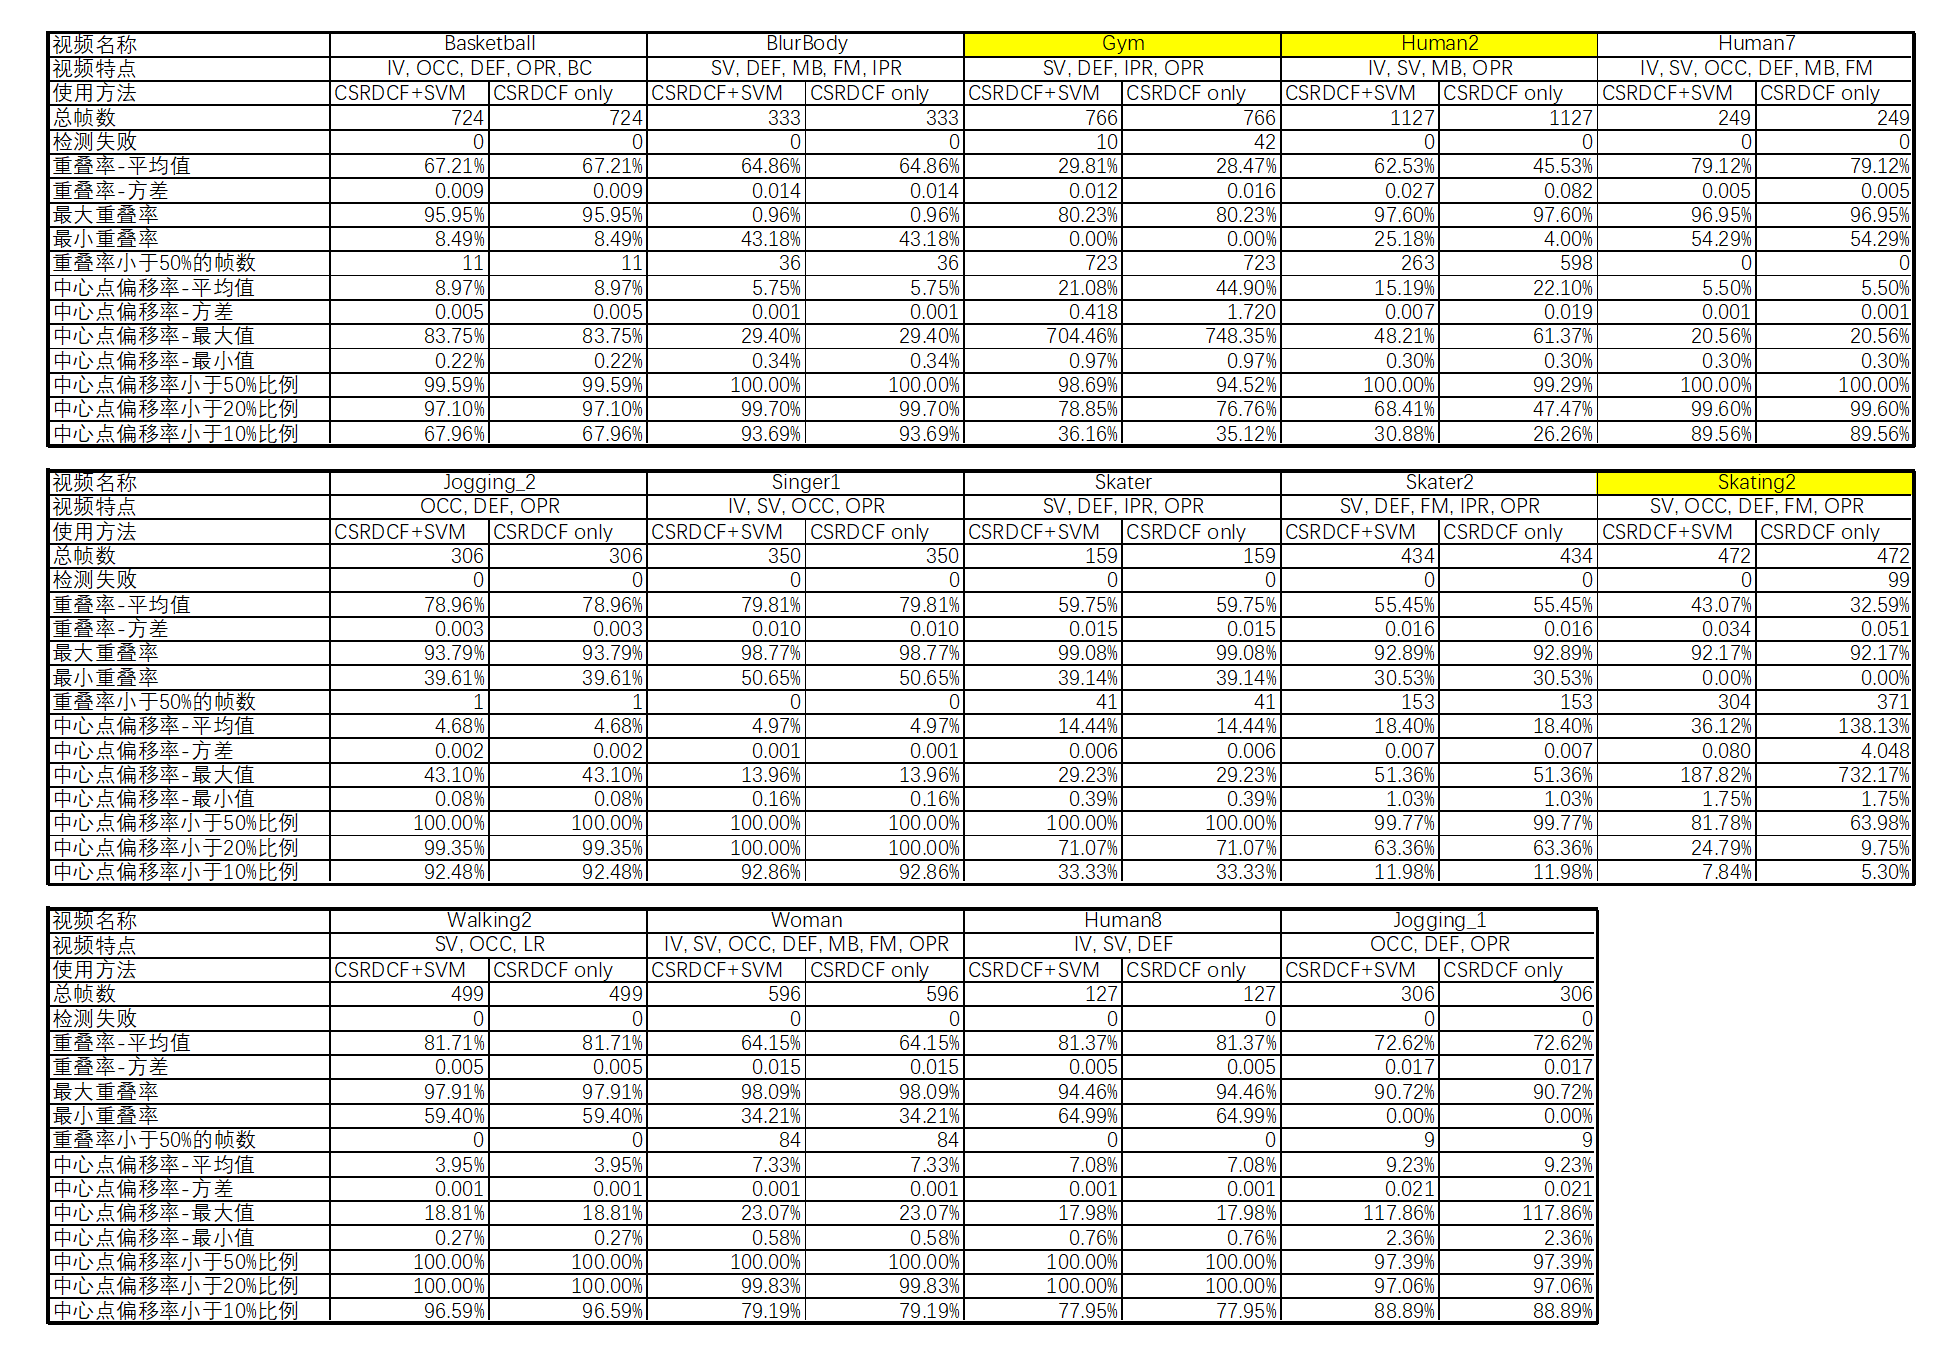
\includegraphics[width=1.1\textwidth]{result.png}
  \caption{详细实验数据}
  \label{fig:results}
\end{figure}




\backmatter
% !TeX root = ../main.tex

\begin{acknowledgements}

在研究学习期间,我有幸得到了三位老师的教导,
他们是:我的导师,中国科大XXX研究员,中科院X昆明动物所马老师以及美国犹他大学的XXX老师。
三位深厚的学术功底,严谨的工作态度和敏锐的科学洞察力使我受益良多。
衷心感谢他们多年来给予我的悉心教导和热情帮助。

感谢XXX老师在实验方面的指导以及教授的帮助。
科大的XXX同学和XXX同学参与了部分试验工作,在此深表谢意。

\end{acknowledgements}

% !TeX root = ../main.tex

\begin{publications}

\section*{已发表论文}

\begin{enumerate}
\item A A A A A A A A A
\item A A A A A A A A A
\item A A A A A A A A A
\end{enumerate}

\section*{待发表论文}

\begin{enumerate}
\item A A A A A A A A A
\item A A A A A A A A A
\item A A A A A A A A A
\end{enumerate}

\section*{研究报告}
\begin{enumerate}
\item A A A A A A A A A
\item A A A A A A A A A
\item A A A A A A A A A
\end{enumerate}

\end{publications}


\end{document}
